\documentclass[12pt, a4paper]{article}

\usepackage[utf8]{inputenc}
\usepackage[russian]{babel}
\parindent 0pt
\parskip 8pt
\usepackage{amsmath}
\usepackage{amssymb}
\usepackage{array}
\usepackage{floatrow}
\usepackage{float}
\usepackage[left=2.3cm, right=2.3cm, top=2.7cm, bottom=2.7cm, bindingoffset=0cm]{geometry} % headheight=0pt,
\usepackage{hyperref}
\usepackage{graphicx}
\usepackage{multicol}
\usepackage{fancyhdr} 
\usepackage{extramarks}
\usepackage[usenames,dvipsnames]{color}
\usepackage{titlesec}
\usepackage{tikz}
\definecolor{grey}{RGB}{128,128,128}

\pagestyle{fancy}
\fancyhf{}
\lhead{Билет № 2.6}
\chead{Процессоры: общего назначения/потоковые, ядра/многопроцессорные системы, одновременная многопоточность (SMT, HT)}
\rhead{\thepage}
\lfoot{made with Ы}
\cfoot{}
\rfoot{\today}
\renewcommand\headrulewidth{0.4pt}
\renewcommand\footrulewidth{0.4pt}

\titlespacing*{\section}{0pt}{5pt}{0pt}
\titlespacing*{\subsection}{0pt}{5pt}{0pt}
\titlespacing*{\subsubsection}{0pt}{5pt}{0pt}

\begin{document}
\section{Прерывания\textasciicircum}
\textbf{Прерывание} (\textit{interrupt}) - сигнал процессору о событии, которое требует его внимания. Процессор отвечает на сигнал прерывания, останавливая выполнение текущей задачи, сохраняя её состояние и вызывает \textbf{обработчик прерываний} (\textit{interrupt handler)}.\\
\textbf{Аппаратное прерывание} используется устройствами чтобы сообщить о том, что им требуется внимание со стороны операционной системы. Например, нажатие клавиши на клавиатуре вызывает прерывание, после чего процессор считывает, какая клавиша была нажата, а затем продолжает выполнение.\\
\textbf{Программное прерывание} вызывается программным исключением (например, делением на ноль) или специальной инструкцией, которая вызывает прерывание при исполнении.\\
\section{Вытесняющая многозадачность}
ОС через некоторый промежуток времени прерывает выполнение одной задачи и переключается на следующую. Таким образом создаётся впечатление многозадачности на одном вычислителе.\\
\section{Про процессы}
\textbf{Процесс} - экземпляр компьютерной программы, запущенный на выполнение. У каждого процесса своя память и свои права.\\
\textbf{Тред} - наименьшая последовательность инструкций, которая может независимо управляться планировщиком. У каждого треда свои регистры (IP и общего назначения), свой выделенный стек в общей для процесса оперативной памяти (треды не пересекаются).\\
\begin{figure}[h]
    \centering
    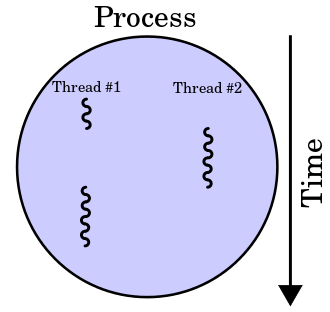
\includegraphics[width=0.4\linewidth]{images/process.png}
    \caption{Жизнеутверждающая картинка: Процесс с двумя тредами, запущенными на одном процессоре}
    \label{fig:Process}
\end{figure}
Теперь распределение памяти происходит на уровне процессов, а распределение вычислительной мощности - на уровне тредов. Но чтобы вся эта прелесть работала и давала ускорение, нужно, во-первых, чтобы задачу вообще можно было распараллелить, а во-вторых, программисту нужно правильно написать.
\subsection{Закон Амдала*}
Закон Амдала - формула, позволяющая предположить теоритическое ускорение программы при исполнении её на нескольких вычислителях.\\
В общем виде звучит как-то так: "Вне зависимости от числа вычислителей, минимальное время исполнения программы не может быть меньше, чем время, необходимое для выполнения той части программы, которую нельзя распараллелить". По это причине параллельные вычисления дают сильный выигрыш в скорости только для задач, которые хорошо параллелятся. Т.е. тогда, когда у нас много независимых вычислений.
\section{SMT/HT}
\textbf{SMT} - \textit{Simultaneous multithreading} - техника, улучшающая эффективность работы суперскалярной архитектуры. Один физический CPU притворяется двумя логическими. Треды независимы, поэтому планировщику проще найти независимые команды, следовательно конвееры эффективнее используются.\\
\textbf{HT} - \textit{Hyperthreading} - SMT у Intel.
Ядро с SMT должно иметь больше регистров (отдельные для каждого треда).\\
В лучшем случае мы можем получить выигрыш в два раза. В худшем треды могут "подраться" за ресурсы. Например, за кэш.\\
Выигрыш от SMT получается, если:
\begin{itemize}
    \item Тредов больше, чем физических ядер
    \item Каждый тред "написан не очень хорошо", т.е. не по максимуму использует конвееры.
\end{itemize}
\section{\textasciicircum}
\begin{itemize}
    \item \textbf{SISD} (\textit{Single Instruction stream, Single Data stream}) - к этой категории относятся компьютеры, которые для программиста выглядят как реализующие только последовательное выполнение. Однако, на уровне микроархитектуры может использоваться ILP.
    \item \textbf{SIMD} (\textit{Single Instruction stream, Multiple Data stream}) - Одни и те же инструкции выполняются над разными данными. Такой подход используется в GPU и в векторных архитектурах.
    \item \textbf{MISD} (\textit{Multiple Instruction stream, Single Data stream}) - коммерческих процессоров такого типа не существует, но идея прикольная.
    \item \textbf{MIMD} (\textit{Multiple Instruction stream, Multiple Data stream}) - Каждый исполнитель выполняет собственную программу над собственными данными. Параллелизм уровня тредов.
\end{itemize}
\section{Мультипроцессорный vs мультиядерный}
Процессор - весь чипсет.\\
Ядро - вычислитель, обычно у ядра свой L1 и L2 кэш, а L3 общий со всеми ядрами.
\section{Видеокарточки}
\subsection{Поток сознания}
В начале времен видеокарточка была просто контроллером памяти: переводила данные из видеопамяти в аналоговый сигнал для ЭЛТ-монитора.\\
А потом стали популярны окошечные интерфейсы типа Windows 3. В чем проблема? Нужно заливать цветом большие области. Программно так делать можно было, но лагало (т.к. процессор занимался рисованием окошечек вместо полезных дел). Чтобы не лагало, появились первые 2D-ускорители.\\
2D-ускоритель - специальный блок на видеокарточке, который умел выполнять операции вида "залить блок таким-то цветом".\\
С другой стороны, появился разный САПР (система автоматизированного проектирования) софт, который позволял смотреть на чертежи в 3D. Но этим САПРам требуется много чего считать с плавающей точкой.\\
\textit{Откуда взять storytelling? - Выкинуть функан.}\\
3D-ускорители аппаратно делали необходимые вычисления, но стоили дико дорого и встречались в специализированном железе.\\
3dfx - выпустила на рынок дешевый аппаратный 3D-ускоритель Voodoo.\\
\textit{Вставьте сюда вашу любимую байку про DOOM.}\\
Как выглядела Voodoo: отдельное устройство, один провод от видеокарточки, другой в монитор. Эта штука умела только в 3D, причем только в полноэкранный.\\
3dfx - появилась технология SLI: возможность использовать две карточки, одна будет считать четные строки, другая нечетные.\\
\textit{Вставьте сюда рандомный срач про игрушки}
\subsection{OpenGL \& DirectX}
OpenGL - 3D API для рассчетов всякого разного 3D.\\
DirectX - 3D API от Microsoft, смысл которого - захватить мир.\\
\subsection{Продолжение потока}
Через некоторое время стало понятно, что аппаратно реализовать все извращения, которые хочется игрописателям, не представляется возможным, т.к. их слишком много. Очевидное решение: сделать часть процесса 3D-проектирования программным. Программные кусочки получили название \textbf{шейдеры}.\\
Исходно было два вида шейдеров: пиксельные и вершинные.\\
Вершинные (вертексные) отвечали за геометрию, пиксельные (фрагментные) - за закраску геометрии (текстурами, например).\\
Шейдеры позволили делать более хитрое освещение и т.п.\\
Исходно в видеокарточке половина блоков считала вершинные шейдеры, половина - пиксельные. Но была проблема в том, что игры неравномерно использовали шейдеры. (Есть два способа нарисовать кружочек: сделать много треугольничков(нагрузка на вершинные) или сделать два треугольничка, но сложную текстуру с прозрачностью(нагрузка на пиксельные)).\\
Со временем сделали универсальные вычислительные блоки.
\subsection{GPGPU}
\textbf{В видеокарточках нет одной из важных возможностей процессора - аппаратного разграничения доступа.}\\
\textit{Вставьте сюда кулстори про Meltdown.}\\
По уровню вычислительной гибкости карточки почти дошли до уровня процессоров. В результате их стали пытаться использовать в качестве GPGPU.\\
\textbf{GPGPU} (\textit{General Purpose computing on GPU} - вычисления общего вида на видеокарточках, не обязательно графика.\\
Сначала это работало так: рисовался прямоугольничек, создавались текстуры, в которые заливались текстуры входных данных), потом с помощью пиксельных шейдеров эти текстуры накладывались так, чтобы всё считалось как надо. Выходные данные тоже записывались в текстуру.\\
Далее стали появляться различные API, которые стали позволять считать не-графику на видеокартах с меньшим количеством извращений.\\
\textbf{CUDA} - платформа и API от NVIDIA, которая позволяет вставить в код конструкции со смыслом "а вот это посчитать на видеокарточке". Потом этот код разбивается на две части: одна компилится вашим компилятором для исполнения CPU, другая компилится под видеокарточку компилятором NVIDIA. В итоге получается код, зависимый от библиотек NVIDIA.\\
\textit{Место для байки про захват мира и NVIDIA}\\
\textbf{OpenCL} - открытый стандарт, который проспонсировали Apple.\\
\section{Различия CPU от GPU}
В у нас есть много однотипных вычислений над разными точками. И эти вычисления выглядят как треды, выполняющие один и тот же код, но над разными данными (SIMT). Вместо того, чтобы создать цикл по всем точкам изображения, создаём много тредов, каждый из которых считает одну точку.\\
Следовательно, у нас есть много независимых вычислений. Кроме того, нас не интересует время выполнения одного треда, а только \textit{выполнение всех тредов в целом}.\\
Если много тредов, то имеет смысл сделать много простых ядер. Т.к. нас не интересует время выполнения одного треда, то мы можем сэкономить на некоторых штуках, которые нам это время оптимизировали. Во-первых, можно выкинуть кэш (т.к. lattency решается по-другому). Во-вторых, можно выкинуть планировщик. В-третьих, можно выкинуть всю невычислительную логику, например, предсказатели переходов.\\
Как решить проблему с долгим откликом памяти? На каждом ядре запустить много-много тредов. Как это работает: ядро начинает исполнять первый тред, исполняет, пока не случается обращение к памяти, ядро посылает команду обращения к памяти и переходит к следующему треду и т.д.\\
Ключевая разница с SMT: логически SMT исполняет два треда и физически исполняет два треда, а в потоковом ядре логически исполняется 16 тредов, а физически только один.
\end{document}